\section*{Appendix}
\addcontentsline{toc}{section}{Appendix}

\subsection*{Code}
De python code die schreven is voor dit model is staat in een GitHup repository.\\
Deze is te vinden via de volgende link: 
https://github.com/bverhage/Algae\\
\\
Door de grootte van de code is er gekozen om de code te verdelen over verschillende documenten. Om de in dit verslag gebruikte resultaten te zien en de simulatie te runnen hoeft enkel het bestand met de naam 'Execution.py' gerund te worden. Een verdere beschrijving van de code staat op de GitHup webpagina.
\cite{artikel1}
\newpage
\subsection*{Testen stabiliteits-voorwaarde a.d.h. numerieke oplossing rond de evenwichts-oplossing}
In deze sectie zullen 2 tijdstap afschattingen grafisch gecheckt worden. Als we $A$ gelijk kiezen aan 0.7 zal de tijdstap kleiner 0.78 dagen.

\begin{figure}[H]
  \centering
  \makebox[\textwidth][c]{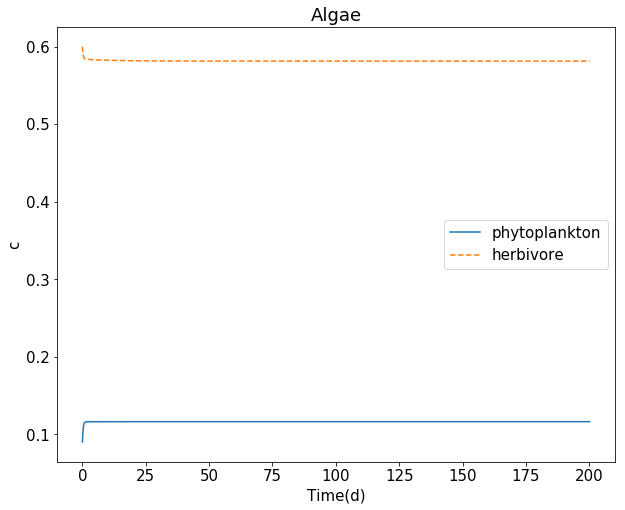
\includegraphics[width=0.4\textwidth]{figures/appendixstab/dt02.png}
  \hfill
  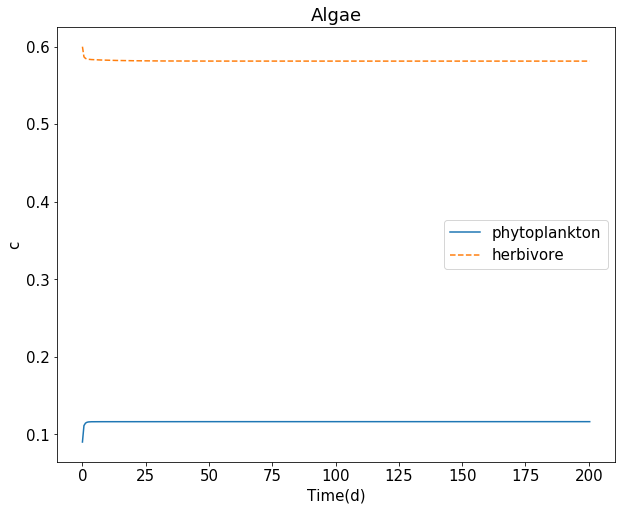
\includegraphics[width=0.4\textwidth]{figures/appendixstab/dt06.png}
  \hfill
  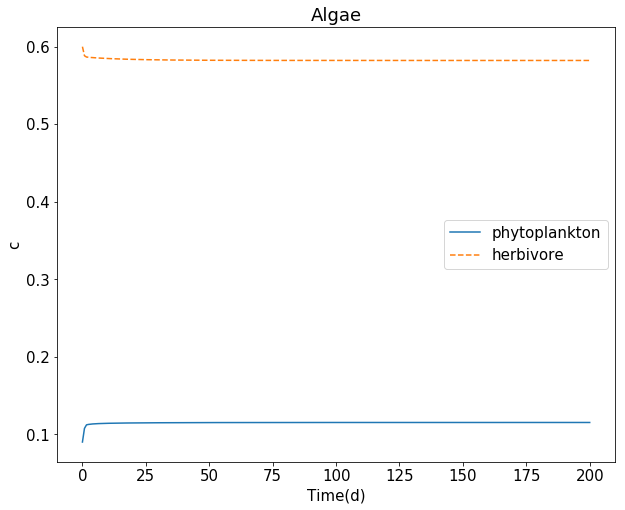
\includegraphics[width=0.4\textwidth]{figures/appendixstab/dt08.png}
    }
  \\
  (a):$\Delta t=0.2$ \hspace{0.27\textwidth} (b):$\Delta t=0.6$\hspace{0.27\textwidth}(c):$\Delta t=0.8$
  \makebox[\textwidth][c]{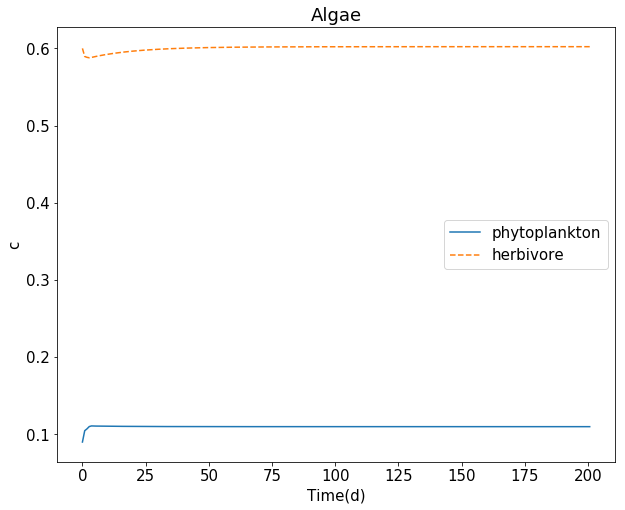
\includegraphics[width=0.4\textwidth]{figures/appendixstab/dt09.png}
  \hfill
  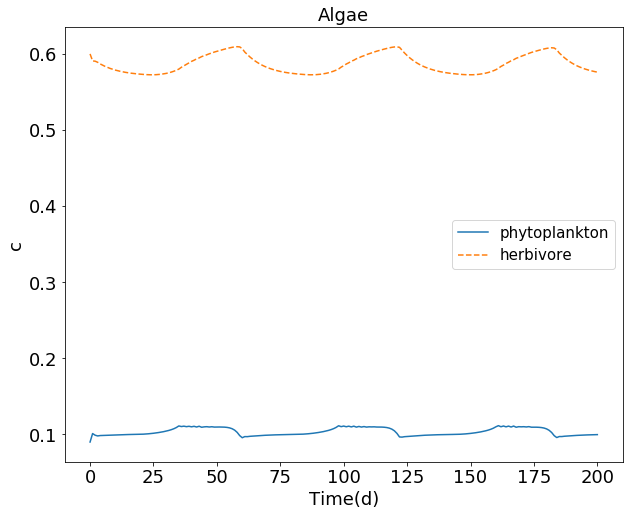
\includegraphics[width=0.4\textwidth]{figures/appendixstab/dt1.png}
  \hfill
  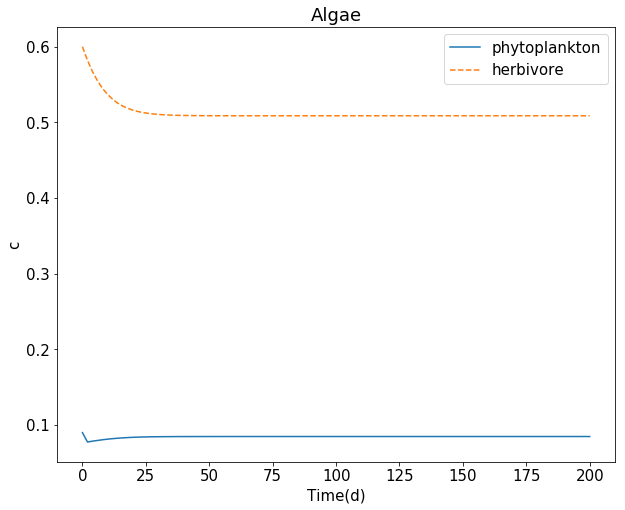
\includegraphics[width=0.4\textwidth]{figures/appendixstab/dt2.png}
    }
  \\
  (d):$\Delta t=0.9$ \hspace{0.28\textwidth} (e):$\Delta t=1$\hspace{0.28\textwidth}(f):$\Delta t=2$
  \centering
  \makebox[\textwidth][c]{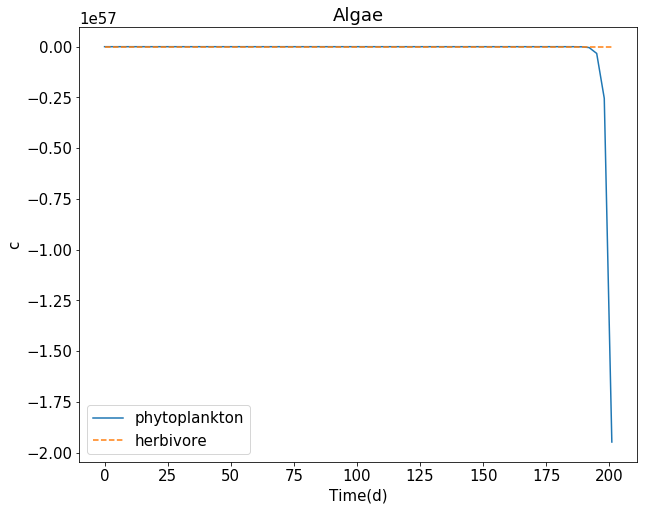
\includegraphics[width=0.42\textwidth]{figures/appendixstab/dt3.png}}
  (g):$\Delta t=3$
  \caption{Oplossingen van het gereduceerde model met een constante $\alpha(t)$, de constante waarde: $A=0.1$. Weergegeven zijn de concentratie $C$ van de phytoplankton en de herbivoren. De beginwaarde zijn dicht bij het evenwicht gekozen. De tijdstap is in dagen gegeven.}
  \label{fig:voorbeelden}
\end{figure} 
Oplossingen van het model voor deze tijdstap zijn weergegeven in Figuur \ref{fig:voorbeelden}, de beginwaarden liggen dichtbij het evenwicht. Voor (a),(b) en (c) convergeert de oplossing netjes naar het evenwicht. Bij (d) en (f) is het evenwicht een stukje verschoven van de $"$echte" waarden af. (e) en (g) convergeren duidelijk niet naar een evenwicht en zijn instabiel. Het blijkt dus dat de stabiliteits-voorwaarde redelijk klopt.\\
Voor $A=0.1$ zijn oplossingen weergegeven voor verschillende waarden van de tijdstap $\Delta t$ in Figuur \ref{fig:voorbeelden1}. Voor deze $A$ is het tijdstap criterium: $\Delta t \leq 0.67$. Hier convergeren de oplossingen die voldoen aan dit criterium, (a) en (b), naar het evenwicht. (c) convergeert al niet snel meer naar een evenwicht, het evenwicht is hier ook verschoven. Bij (d) zitten er al wat numerieke artefacten in. In (e) is de oplossing divergent en instabiel. Wederom blijkt de gevonden voorwaarde te kloppen.
\begin{figure}[H]
  \centering
  \makebox[\textwidth][c]{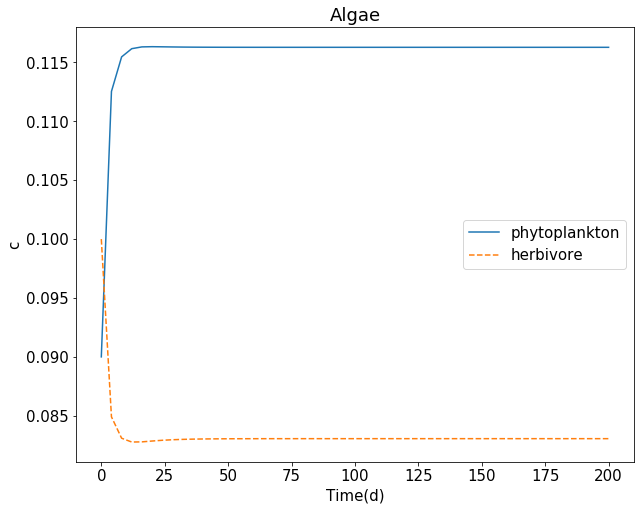
\includegraphics[width=0.4\textwidth]{figures/appendixstab/1dt4.png}
  \hfill
  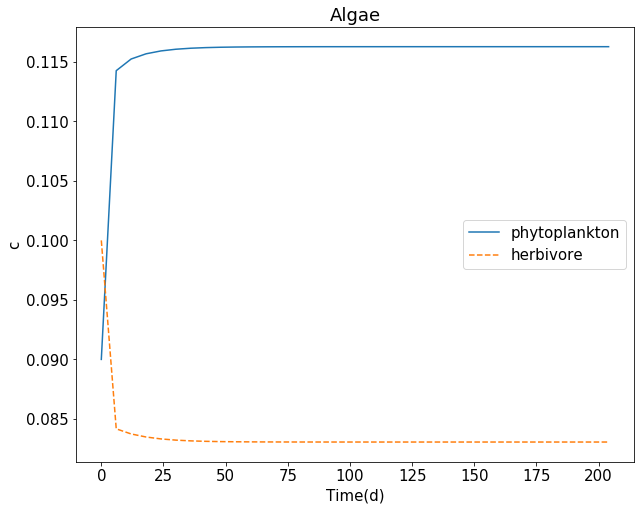
\includegraphics[width=0.4\textwidth]{figures/appendixstab/1dt6.png}
  \hfill
  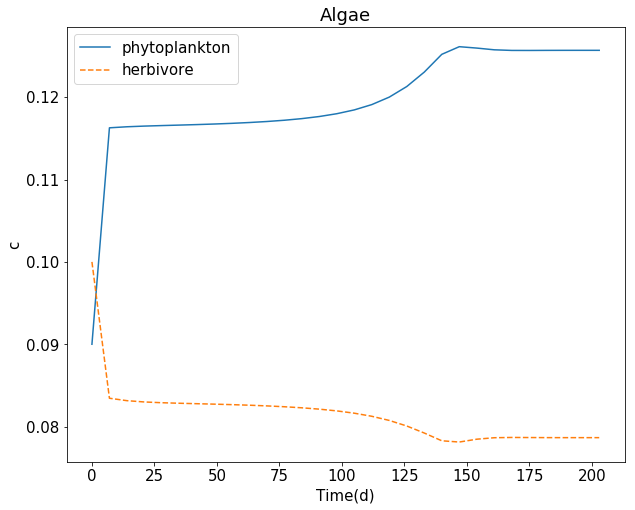
\includegraphics[width=0.4\textwidth]{figures/appendixstab/1dt7.png}
    }
  \\
  (a):$\Delta t=4$ \hspace{0.28\textwidth} (b):$\Delta t=6$\hspace{0.29\textwidth}(c):$\Delta t=7$
  \makebox[\textwidth][c]{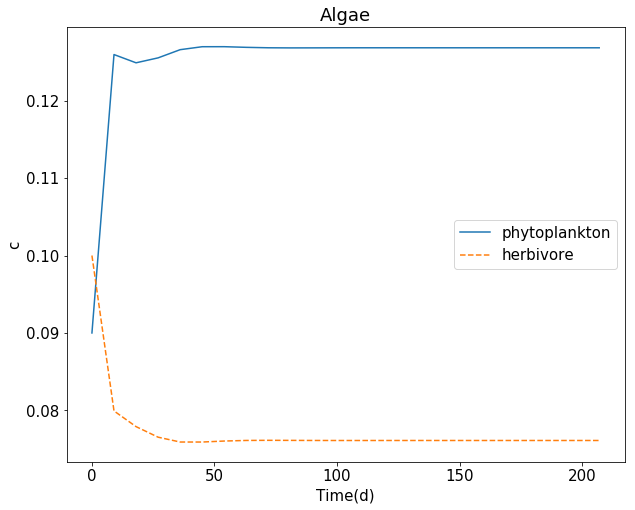
\includegraphics[width=0.4\textwidth]{figures/appendixstab/1dt9.png}
  \hfill
  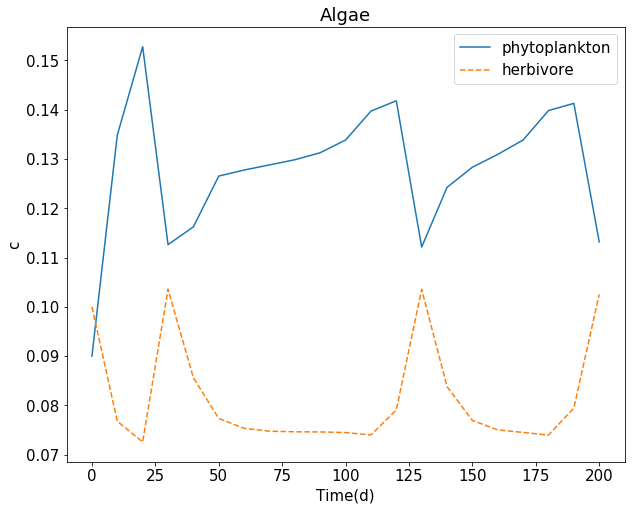
\includegraphics[width=0.4\textwidth]{figures/appendixstab/1dt10.png}
    }
  \\
  \hspace{0.11\textwidth}(d):$\Delta t=9$ \hspace{0.47\textwidth} (e):$\Delta t=10$\hspace{0.1\textwidth}
  \centering
  \caption{Oplossingen van het gereduceerde model met een constante $\alpha(t)$, de constante waarde: $A=0.1$. Weergegeven zijn de concentratie $C$ van de phytoplankton en de herbivoren. De beginwaarde zijn dicht bij het evenwicht gekozen. De tijdstap is in dagen gegeven. De verticale as verandert door de plaatjes heen. }
  \label{fig:voorbeelden1}
\end{figure} 

\newpage

\subsection*{afhankelijkheid fotosynthese van concentratie pythoplankton}

Er zijn verschillende verbanden getest in dit model voor de  afhankelijkheid van fotosynthese snelheid van concentratie pythoplankton. Er is uiteindelijk gekozen voor $\alpha_P=min(\frac{1}{\sqrt[3]{P}},1)$. Aangezien, zoals in figuur \ref{fig:alphavergelijking} te zien, deze een meest vergelijkbaar resultaat geeft met de fotosynthese snelheid uit het verslag van Evans \& Parslow. 

\begin{figure} [H]
    \centering
    \subfloat[]{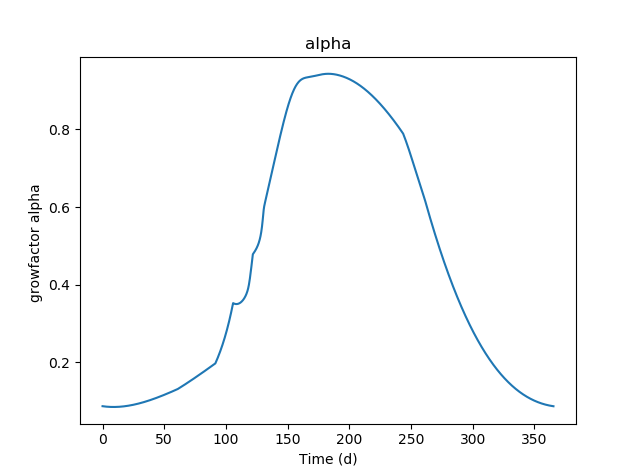
\includegraphics[width=0.35\textwidth]{figures/alpha/aplhaPH4.png}}
    \subfloat[]{\includegraphics[width=0.35\textwidth]{figures/alpha/alphaPH2.png}}
    \subfloat[]{\includegraphics[width=0.35\textwidth]{figures/alpha/AlphaPHe.png}}
    \\
    \subfloat[]{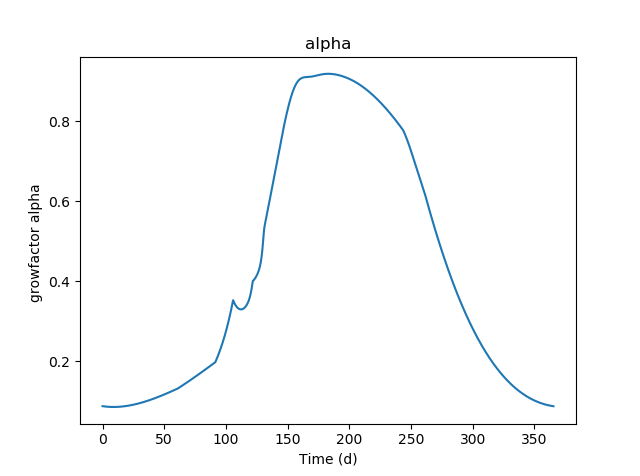
\includegraphics[width=0.4\textwidth]{figures/alpha/alphanormaal2.png}}
    \subfloat[]{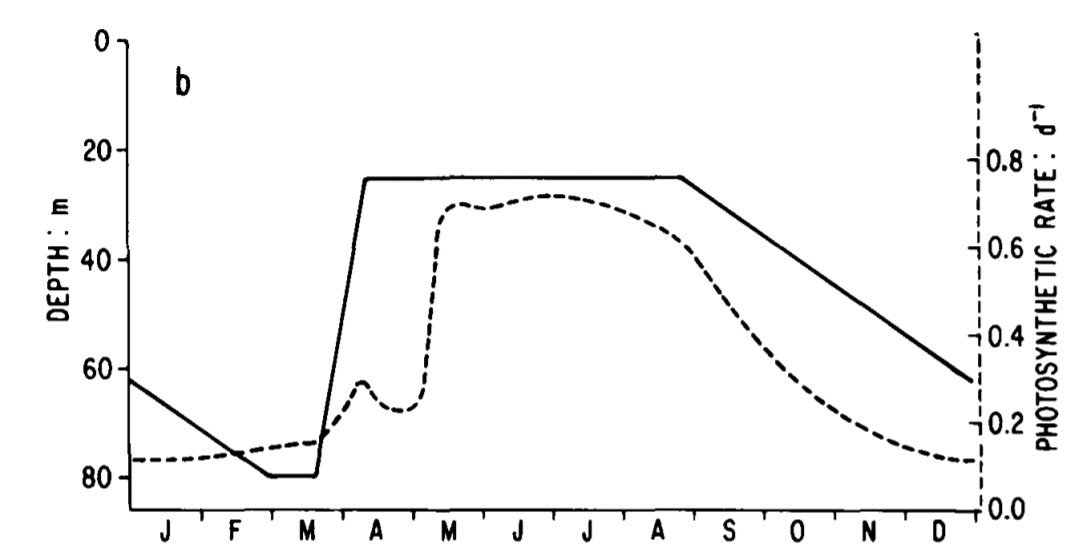
\includegraphics[width=0.5\textwidth]{figures/alpha/evansparslowalpha.PNG}}    
    \caption{  
    (a) De fotosynthese snelheid over tijd voor $\alpha_P=min(\frac{1}{\sqrt[4]{P+H}},1)$  
    (b) De fotosynthese snelheid over tijd voor $\alpha_P=min(\frac{1}{\sqrt[2]{P+H}},1)$  
    (c) De fotosynthese snelheid over tijd voor $\alpha_P=e^{-(P+H)}$ ($\leq 1$ , want $P \geq 0 $)  
    (d) De fotosynthese snelheid over tijd voor $\alpha_P=min(\frac{1}{\sqrt[3]{P+H}},1)$  
    (e) De fotosynthese snelheid over tijd uit het verslag van Evans \& Parslow uit 1985.}
    \label{fig:alphavergelijking}
\end{figure}
